\section{Rigid Body-spring Model for Hybrid connection}

\subsection{Friction type connection}

Since the hybrid connection is composed of a bearing connection and a friction connection, the stiffness of the hybrid connection is determined jointly by the stiffness of the bearing connection and the friction connection. Before calculating the limit state design method for the hybrid connection, the stiffness of the friction connection needs to be calculated first.

\begin{figure}[htbp]
    \centering
    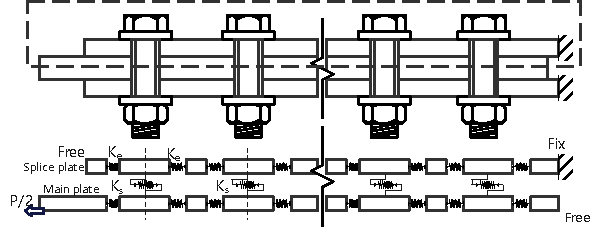
\includegraphics[width=0.8\textwidth]{imgs/ch7/RBSM.pdf}
    \caption{Rigid body-spring model of friction type connection}
    \label{fig-rbsm}
\end{figure}

The stiffness for \ac{RBSM} model of the friction connection can be simplified to the model shown in Fig. \ref{fig-rbsm}, where $k_{s}$ is the stiffness of the friction connection, $k_{e}$ is the stiffness of the steel plate considering the circular holes, and the equations for $k_{s}$ and $k_{e}$ are as follows:

\begin{equation}\label{eq-ks}
    K_{s} = 8GA_{se} \varphi / (t + 2 t_{sp})
\end{equation}

Where, $G$ is the shear modulus, $A_{sq}$ is the effective area of the friction connection, $t$ is the thickness of the main plate, $t_{sp}$ is the thickness of the splice plate, and $\varphi$ is the correction coefficient of shear strain, The geometry of the cut micro-unit and the range of friction influences are determined by taking 0.5 for the case of M22 bolts and 28 mm splice plate thickness for this object.

\begin{figure}[htbp]
    \centering
    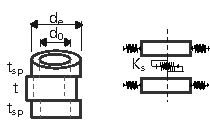
\includegraphics[width=0.8\textwidth]{imgs/ch7/simp_rbsm.pdf}
    \caption{Simple RBSM model under simple shear}
    \label{fig-simp_rbsm}
\end{figure}

As the high-strength bolts through the washer to transfer the clamping force to the friction joint surface as shown in Fig. \ref{fig-simp_rbsm}, so in the consideration of the shear area should be brought into the area of the washer to be considered together, in addition, the actual contact surface pressure range is larger than the washer area, so it is necessary to consider the influence due to the shear strain effect by multiplying a correction coefficient $\psi$ on the washer area $d_w$.
Therefore As can be calculated with the following equation:

\begin{equation}
    A_{se} = \pi{(\psi d_w)^2-d_0^2} / 4
\end{equation}

Where, $d_0$ is the diameter of the bolt hole, and $\psi$ is the correction coefficient of contact area, in the case of thin plates take 1, in the case of thick plates it can be simply taken as 1.4.

\subsubsection{Validation of stiffness calculation}

In order to verify the correctness of the stiffness calculation of the friction connection, the stiffness of the friction connection is calculated by the above formula, and the stiffness of the friction connection is calculated by the Eq. \ref{eq-ks}, and the results are compared with the Chapter 6. 

For the hybrid joint, M22 bolts were used at the end and M16 bolts were used in the middle, and the stiffness of the joint was mainly controlled by the M22 bolts at the end, so when the calculation was carried out, it was agreed to follow the geometry of the M22 bolts at the end in order to facilitate the simplification of the model, and the details of the calculation are shown in Table \ref{tab-calks}.

\begin{table}[]
    \centering
    \caption{Calculation of stiffness of friction type connection}
    \label{tab-calks}
    \begin{tabular}{@{}cccccccc@{}}
    \toprule
     &
      \begin{tabular}[c]{@{}c@{}}Shear Modulus\\ G {[}Gpa{]}\end{tabular} &
      $\psi$ &
      \begin{tabular}[c]{@{}c@{}}$d_w$\\ {[}mm{]}\end{tabular} &
      \begin{tabular}[c]{@{}c@{}}$d_0$\\ {[}mm{]}\end{tabular} &
      \begin{tabular}[c]{@{}c@{}}$A_{se}$\\ {[}$mm^2${]}\end{tabular} &
      $\varphi$ &
      \begin{tabular}[c]{@{}c@{}}$K_s$\\ {[}$kN/mm${]}\end{tabular} \\ \midrule
    M22-bolt &
      77 &
      1.4 &
      44 &
      23.5 &
      2550 &
      0.5 &
      10069.5 \\ \bottomrule
    \end{tabular}
\end{table}

The initial frictional stiffness ks of this hybrid joint is calculated to be 10069 kN/mm. It is assumed here that the friction tends to be horizontal and does not change after sliding of the joint, which is in agreement with the finite element simulation, and therefore the slope is changed to 0 after sliding load. The friction connection can be modeled as the following equation

\begin{equation}\label{eq-nmfc}
    P = \begin{cases}
        K_s \delta, & \text{if } P < F_{s} \\
        F_{s}, & \text{if } P \geq F_{s}
    \end{cases}
\end{equation}

Fig.\ref{fig-ks_compare} represents the comparison made with this model and the experimental results, where NA-FC denotes the numerically Analysis-friction type Connection indicated by the dashed line. This model can be considered as a good simulation of the variation of friction in the joint without considering the preload drop of the bolt.

\begin{figure}[htbp]
    \centering
    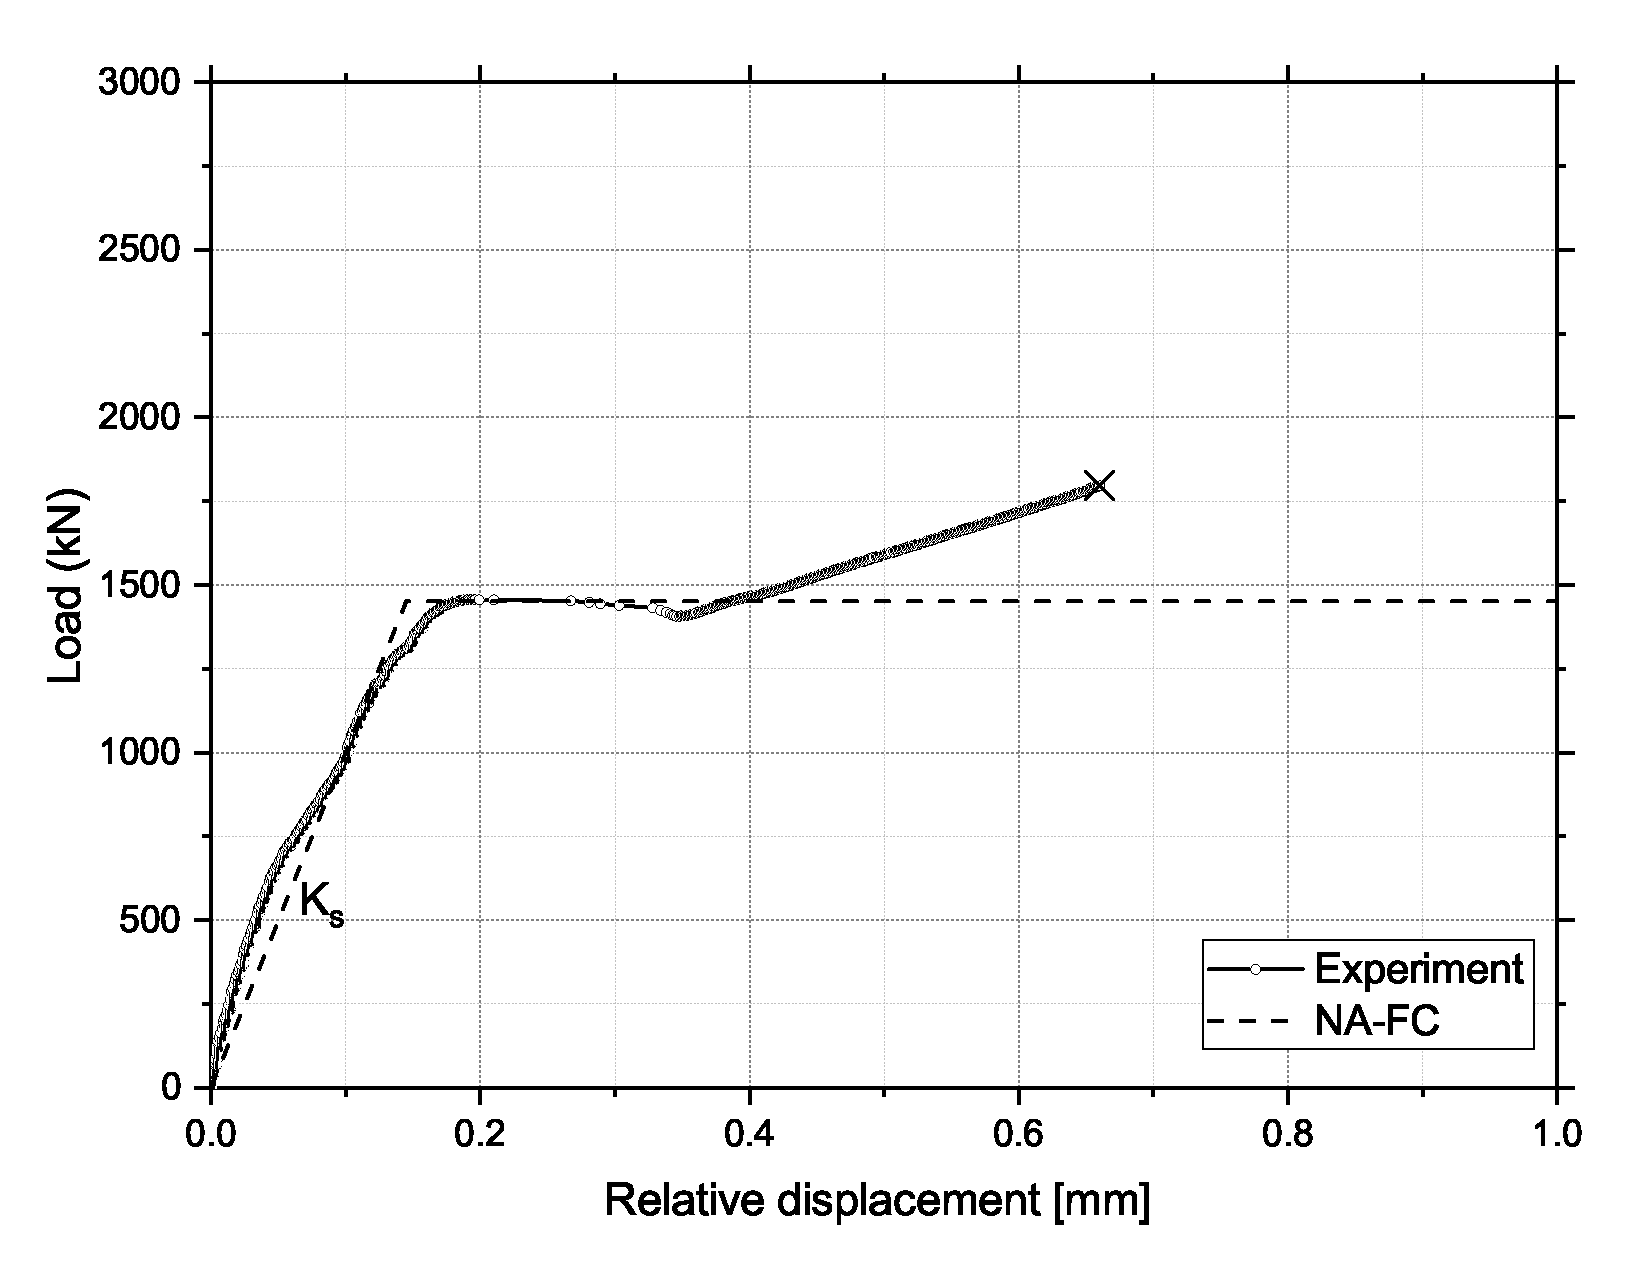
\includegraphics[width=0.7\textwidth]{imgs/ch7/NA-FC.eps}
    \caption{Comparison of stiffness of friction type connection}
    \label{fig-ks_compare}
\end{figure}

\subsection{Bearing type connection}

%对于承压连接,虽然规定了采用承压强度设计时可以不用施加轴力,然而一般设计为了提高刚度和强度,都会对用于承压连接的螺栓施加轴力。这使得承压连接自身就分为了两种状态,一种是不施加轴力的承压连接,一种是施加轴力的承压连接。对于不施加轴力的承压连接,其刚度可以直接通过螺栓的刚度计算得到,而对于施加轴力的承压连接,其刚度需要通过螺栓的剪切和摩擦刚度计算得到。对于,摩擦连接的刚度计算方法已经在上一节中进行了介绍. 因此为了更简单的讨论复合作用下的承压连接的刚度,本节将首先讨论不施加轴力的承压连接的刚度计算方法,然后再讨论施加轴力的承压连接的刚度计算方法。

For pressurized connections, although it is stipulated that no preload can be applied when designing for bearing resistance, the bolts used for pressurized connections are generally designed to apply preload in order to increase stiffness and strength. This makes the bearing connection itself divided into two states, one is the bearing connection without preload, and the other is the bearing connection with preload. For a bearing connection without preload, the stiffness can be calculated directly from the stiffness of the bolts, whereas for a bearing connection with preload, the stiffness needs to be calculated from the shear and friction stiffness of the bolts. For, the stiffness calculation method for friction connections has been described in the previous section. Therefore in order to discuss the stiffness of compression connections under composite action in a simpler way, this section will first discuss the method of calculating the stiffness of compression connections without applied pretension and then the method of calculating the stiffness of compression connections with applied pretension.

\begin{figure}[htbp]
    \centering
    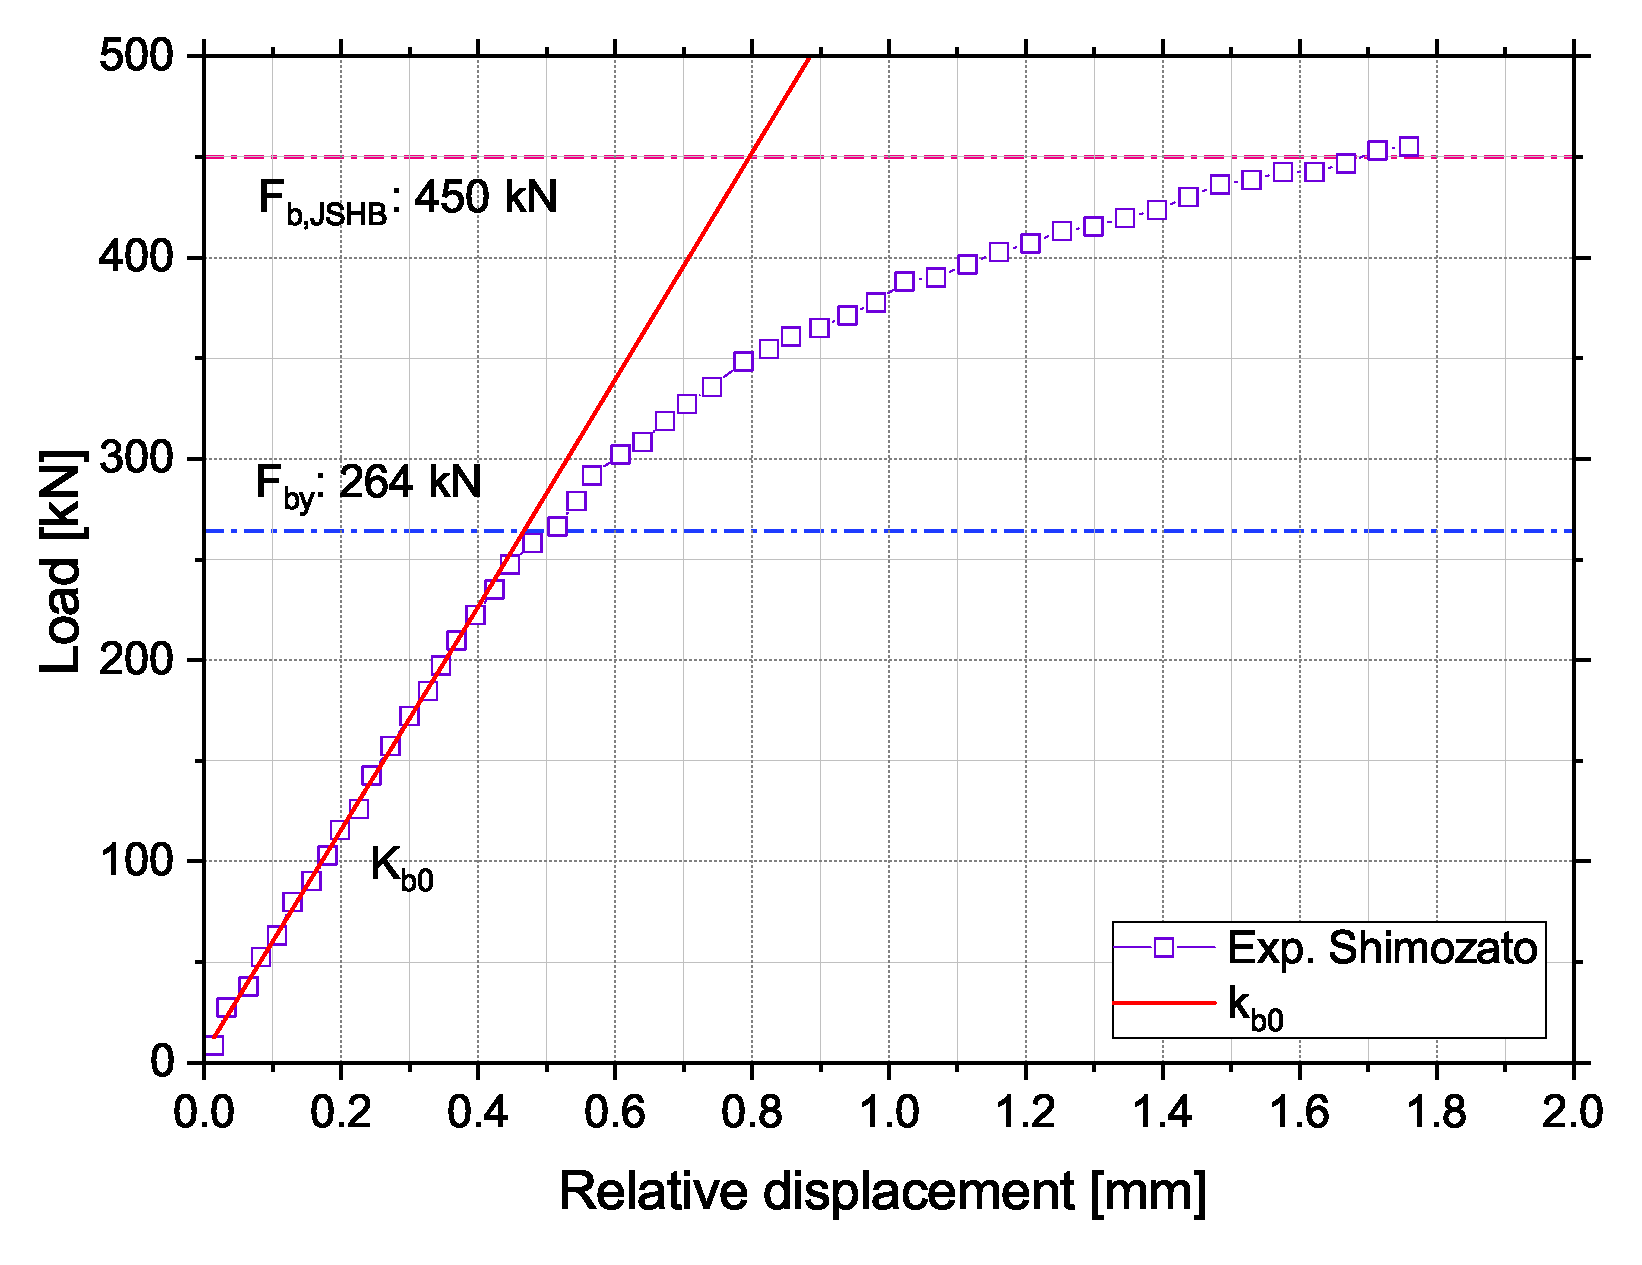
\includegraphics[width=0.7\textwidth]{imgs/ch7/onebbolt.eps}
    \caption{Bearing type connection without pretension}
    \label{fig-onebbolt}
\end{figure}

Fig. \ref{fig-onebbolt} shows the relationship between load and relative displacement for an if bolt subjected to shear with no preload applied. The data were obtained from shimozato's \cite{Shimozato2008ExperrimentalModel} experimental results, and it can be calculated from the experimental results that the bearing connection has an initial stiffness kb0, and the bearing resistance at the service limit strength obtained by the jshb calculation is 450 kN. It has also been mentioned in the previous Chapters \ref{ch4} and \ref{ch6}, respectively, that for the design at the service limit state, the stress-training effect should not be taken into account around the bearing holes, and thus the bearing bearing considered in this study bearing yield resistance $F_{by}$ should be calculated by the following equation:

\begin{equation} \label{eq-fby}
    F_{by} = dtf_y
\end{equation}

The bearing yield resistance obtained from Eq. \ref{eq-fby} is 264 kN, which can be found to be similar to the point in the experimental data where the linear relationship is removed. (purple dotted line and red solid line in the figure)

\subsection{Hybrid connection}

\subsubsection{Simplified theoretical numerical model}

\begin{figure}[htbp]
    \centering
    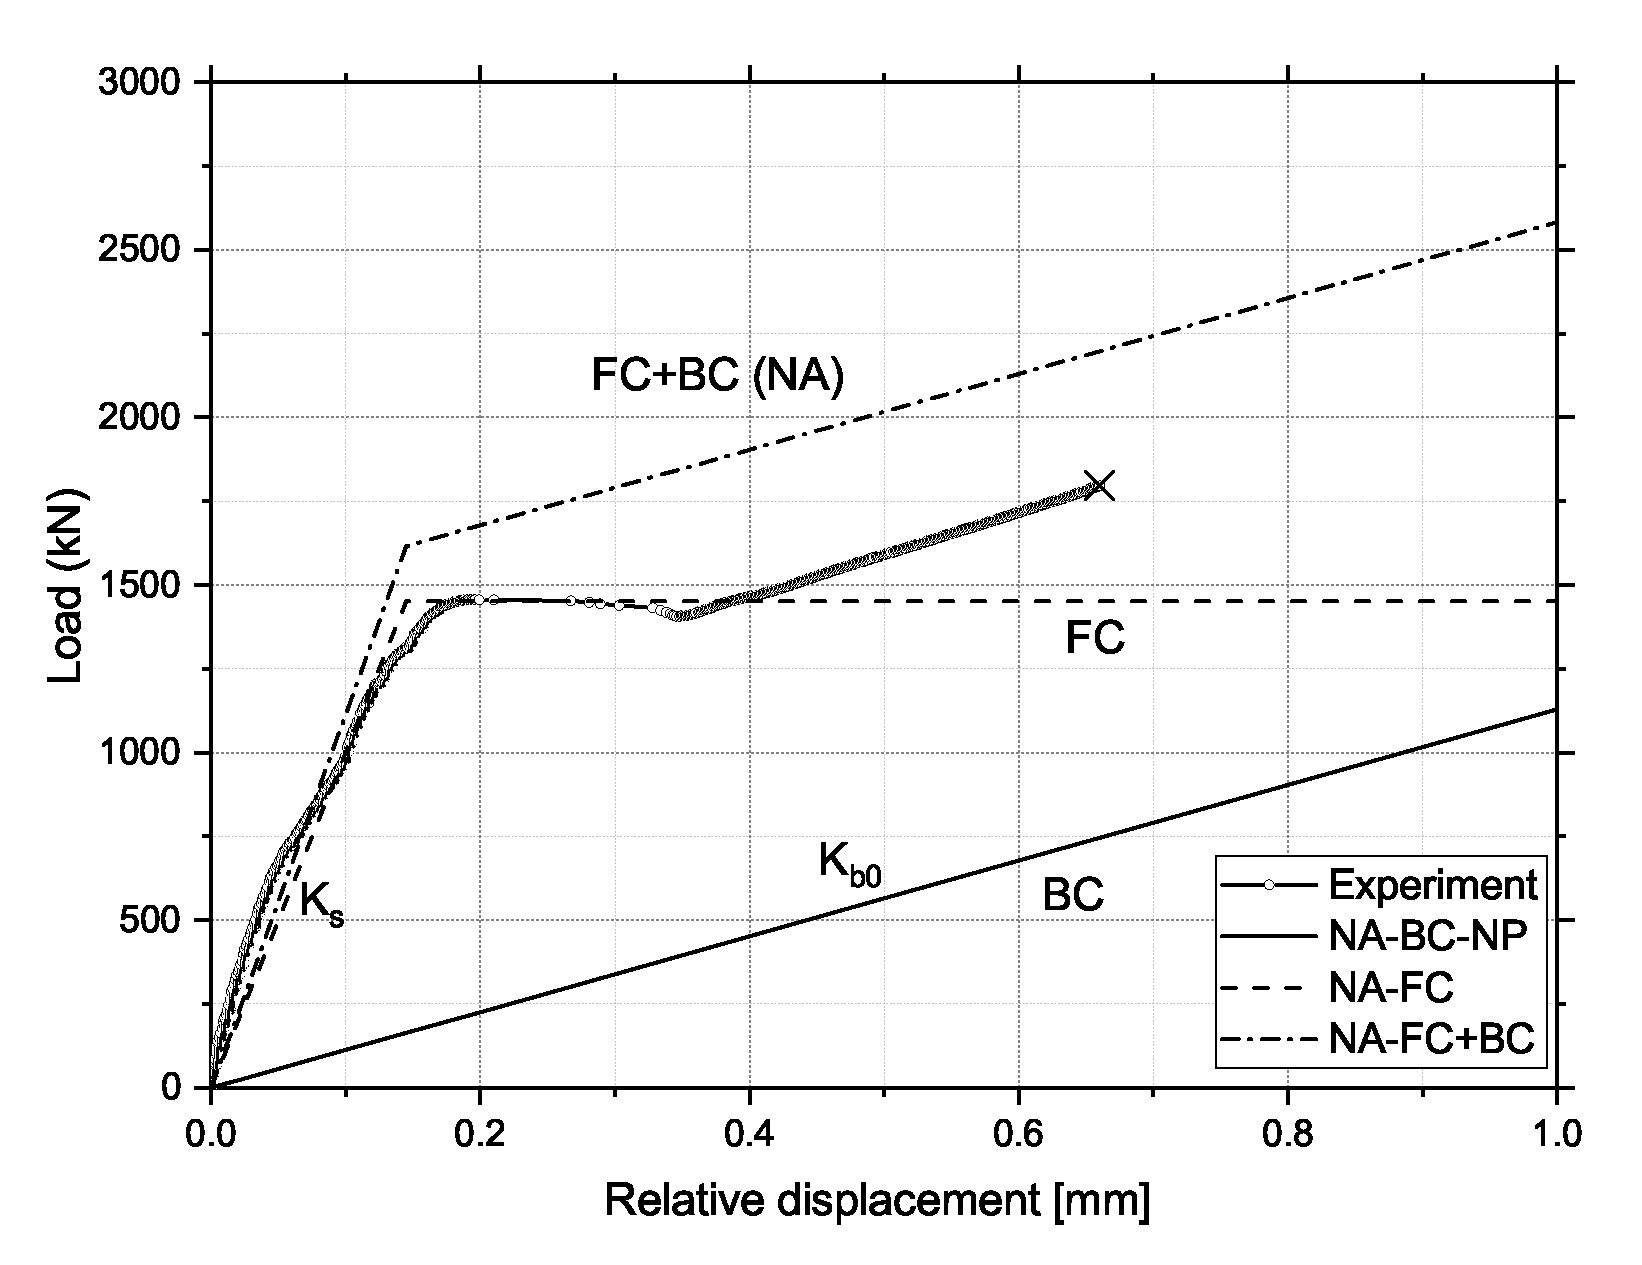
\includegraphics[width=0.7\textwidth]{imgs/ch7/NAFCBC.eps}
    \caption{Simplified theoretical numerical model of hybrid connection}
    \label{fig-nafcbc}
\end{figure}

Fig. \ref{fig-nafcbc} shows the simplified theoretical numerical model obtained by direct summation of the bearing and friction connections, the solid line of BC indicates the initial stiffness of the bearing connection, and the FC is modeled as shown in Eq. \ref{eq-nmfc}. The numerical model obtained by summation can be calculated by the following equation:

\begin{equation}\label{eq-nmhc1}
    P = \begin{cases}
        (K_s + K_{b0}) \delta, & \text{if } P < F_{s} \\
        K_{b0} \delta + F_{s}, & \text{if } P \geq F_{s}
    \end{cases}
\end{equation}

The numerical model simulates only the linear behavior of the hybrid connection, and it can be found that the model has a tendency to have roughly the same behavior as the experimental data for both the primary and secondary slopes, respectively, which can be considered appropriate assuming that no small slips will ideally occur.

\subsubsection{Consider the minor slip}

\begin{figure}[htbp]
    \centering
    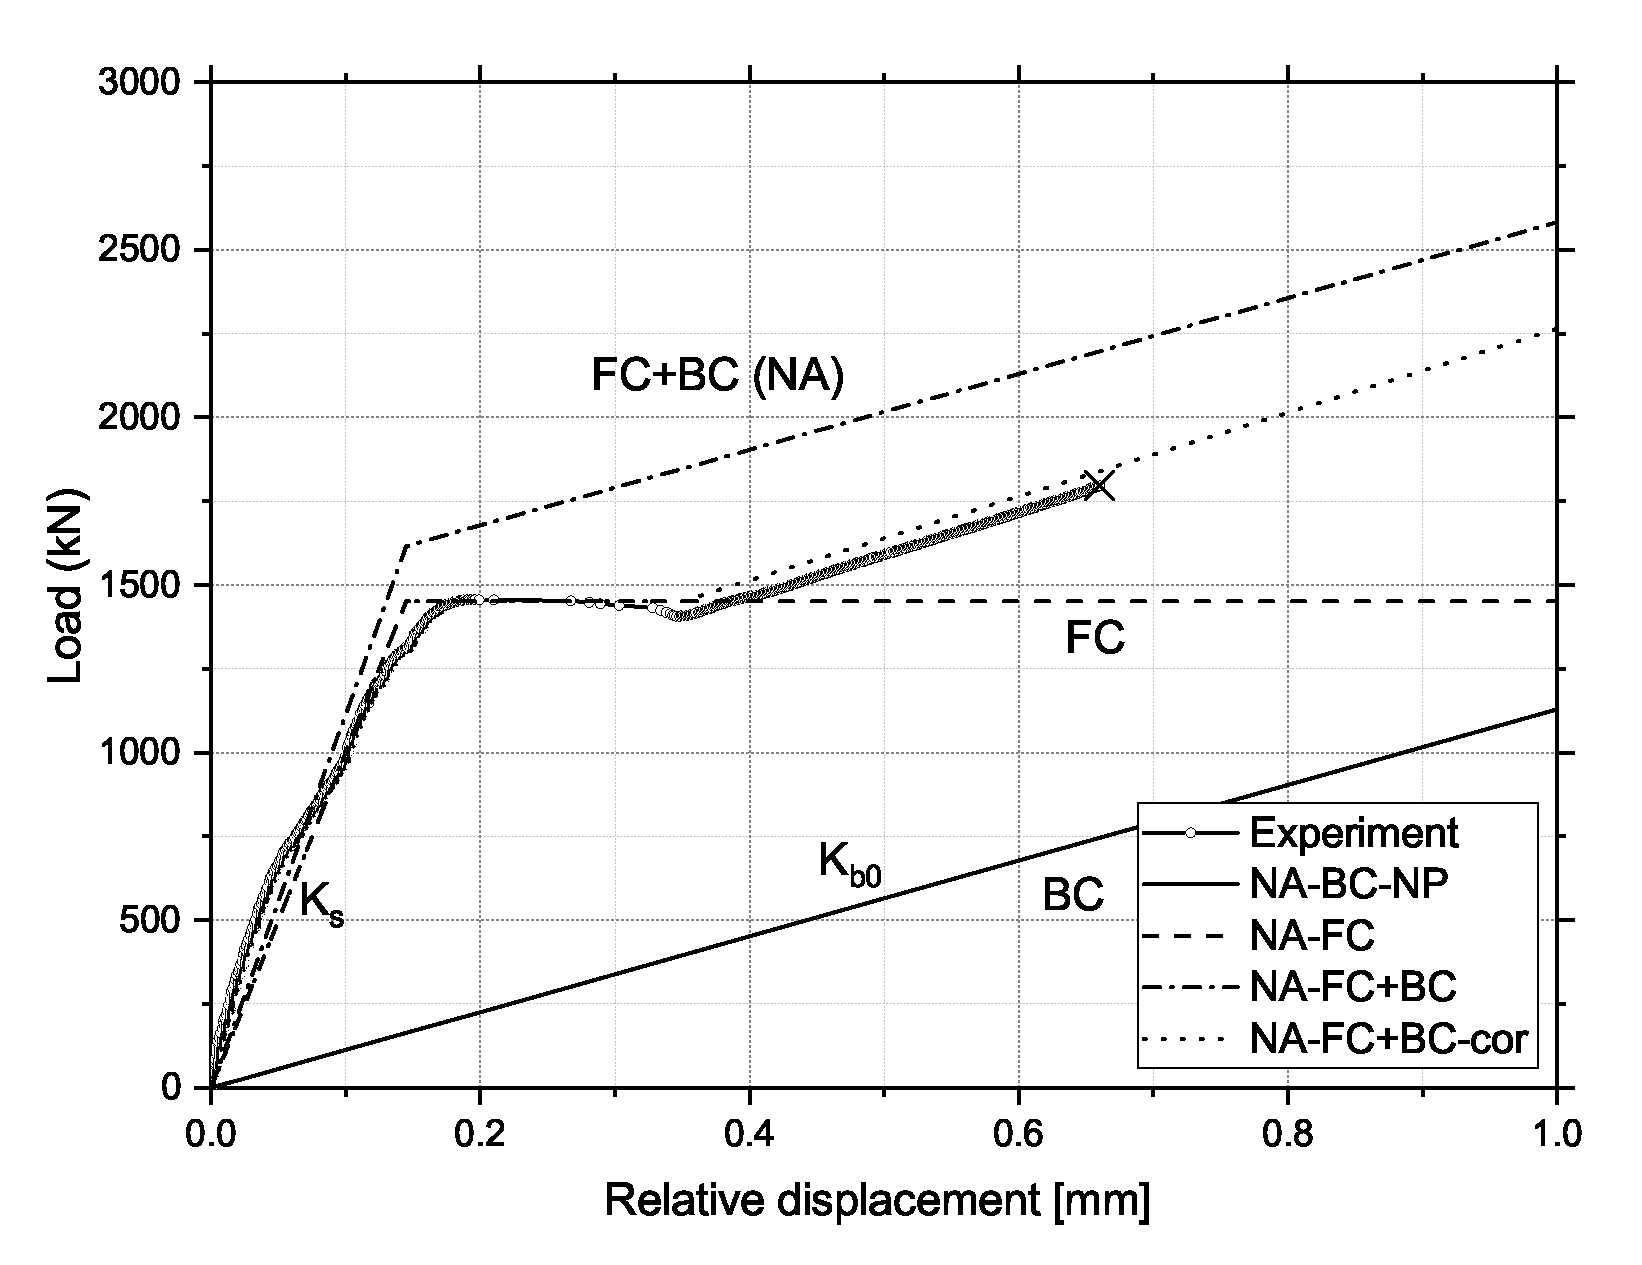
\includegraphics[width=0.7\textwidth]{imgs/ch7/nmfcbc-2.eps}
    \caption{Corrected theoretical numerical model of hybrid connection with minor slip}
    \label{fig-nmfcbc2}
\end{figure}

Fig. \ref{fig-nmfcbc2} represents the model after correction for minor slips based on the base model Eq. \ref{eq-nmhc1}. Considering that at the initial stage of loading, although the bearing will transmit the load together with the friction connection, its load sharing is very small, especially since the initial stiffness of the hybrid connection is almost exclusively affected by the stiffness of the friction connection, this model does not take into account the bearing connection at the initial stage of the friction connection, which is summed up after the occurrence of the small slip. The corrected model is shown below.

\begin{equation}\label{eq-nmhc2}
    P = \begin{cases}
        K_s \delta, & \text{if } P < F_{s} \\
        F_{s}, & \text{if } \delta \leq \delta_{s} \\
        K_{b0} (\delta - \delta_s) + F_{s}, & \text{if } \delta > \delta_{s}
    \end{cases}
\end{equation}

Where, $\delta_s$ is the minor slip value consider the elastic deformation of friction type connection, there take it to 0.35 mm.

The corrected model almost matches the experimental data, in which $\delta_s$, $\delta_s$ consists of the elastic slip of the friction connection, which can be calculated from the stiffness and the slip strength of the friction connection, and the minor slip, which is not easy to recognize because it is impossible to know the amount of the resulting gap. Therefore, for the later evaluation, the main purpose is to discuss how much load reduction factor needs to be set in order to equivalently cancel out the effect of slip for the same amount of displacement as compared to the numerical model in the ideal state.



\subsection{Validation of FE analysis}

Fig. \ref{fig-exp-fem} shows a finite element analysis model of the experimentally validated hybrid-based connection discussed in Chapter \ref{ch6}.

\begin{figure}[htbp]
    \centering
    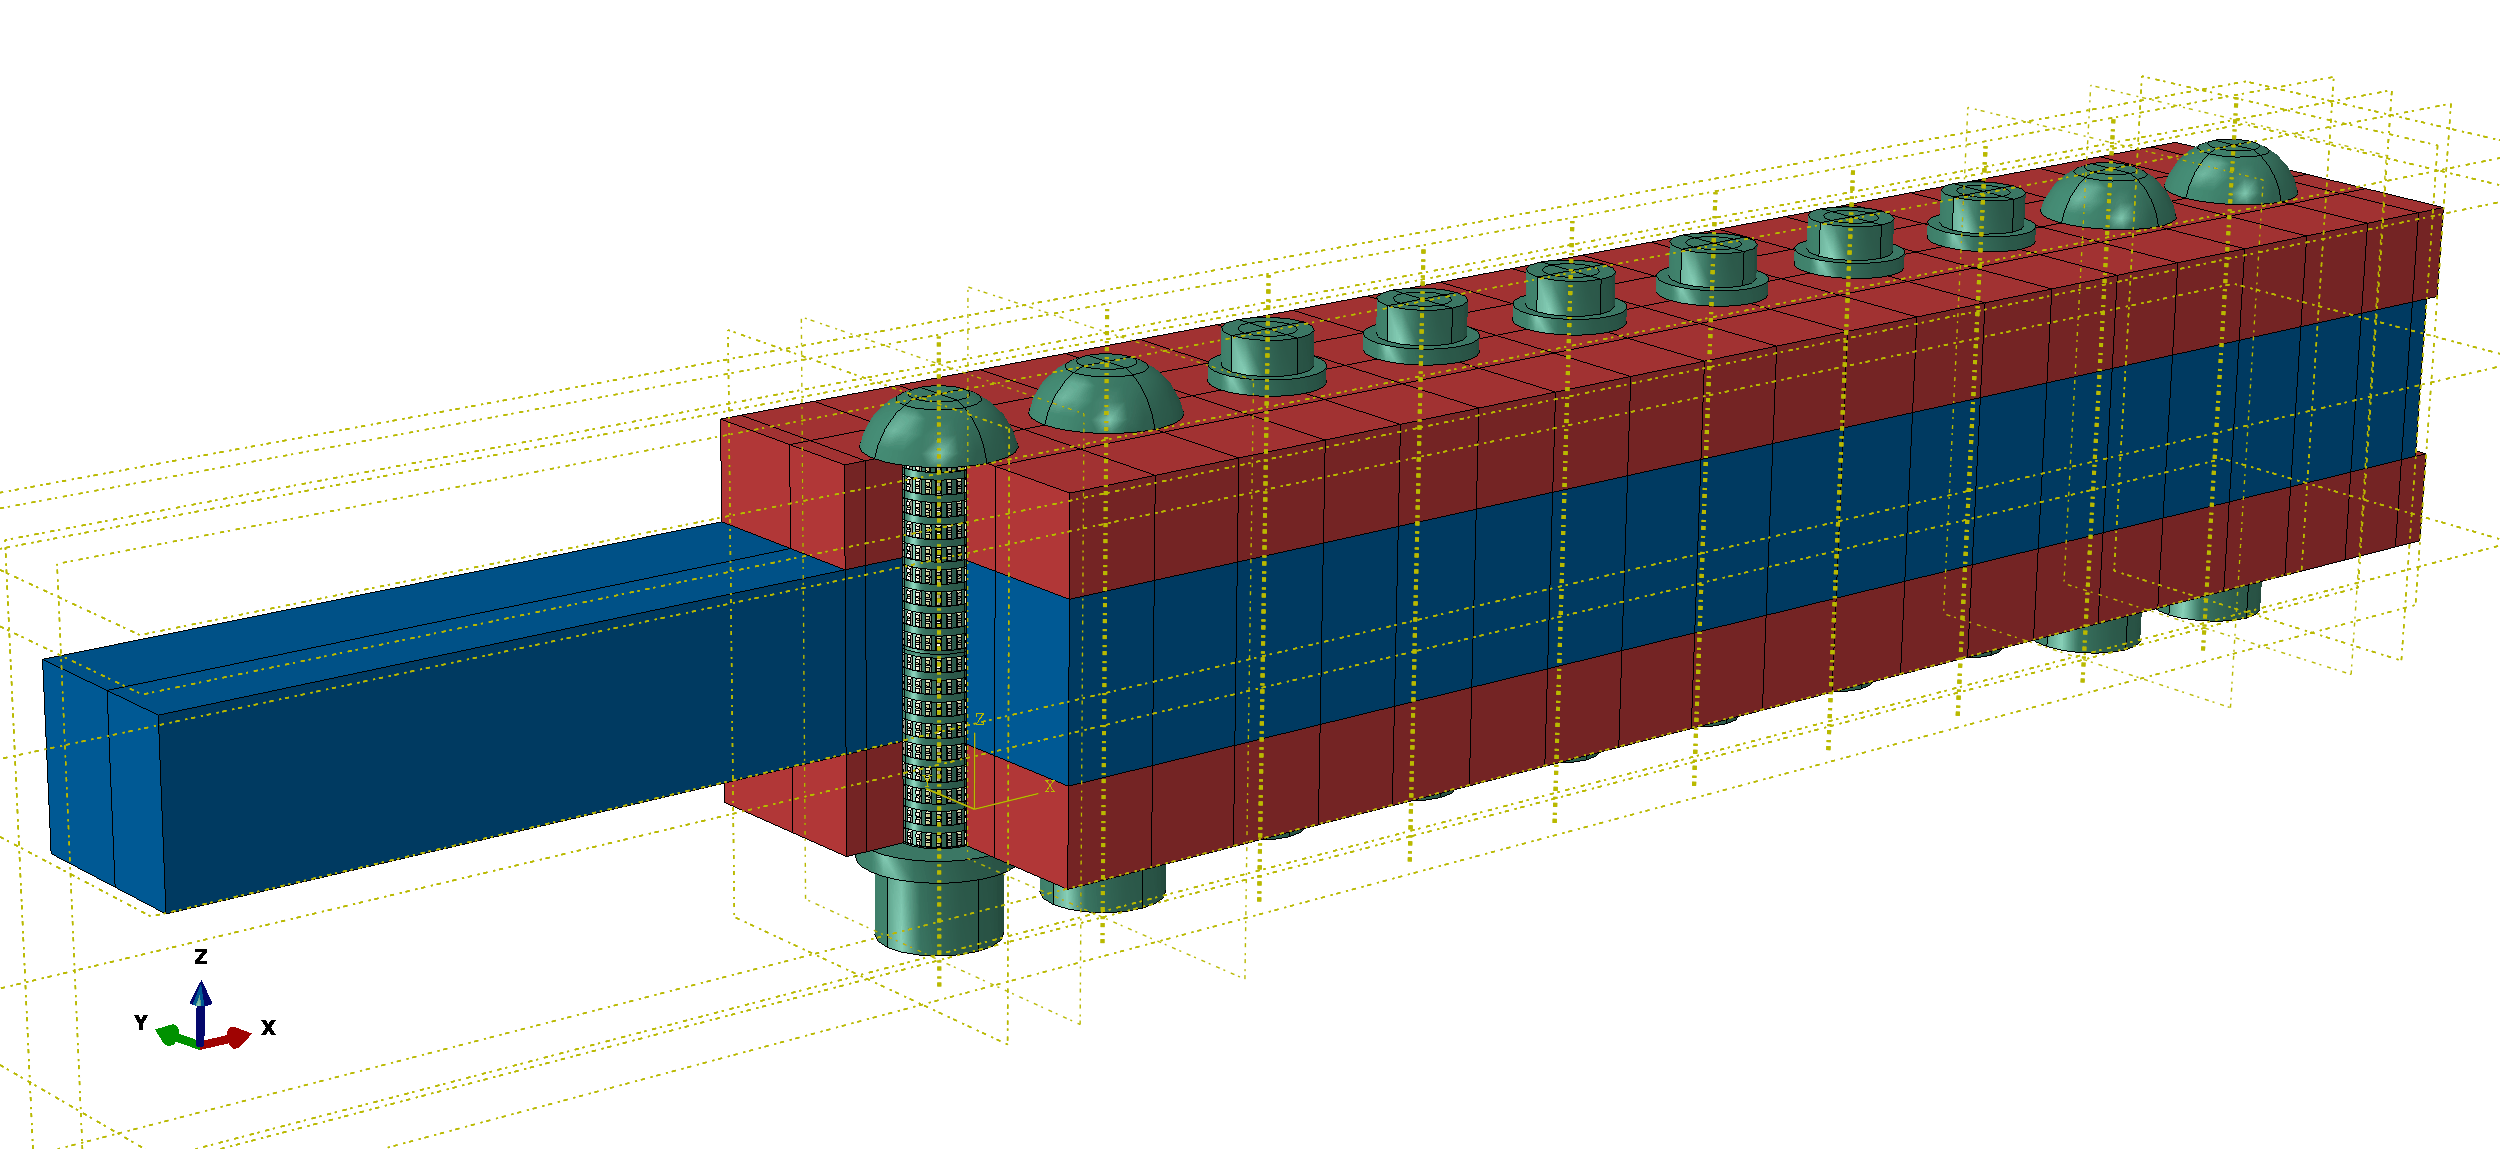
\includegraphics[width=0.8\textwidth]{imgs/ch7/exp-fem.png}
    \caption{FE Model for the experiment hybrid joint}
    \label{fig-exp-fem}
\end{figure}

The geometric dimensions as well as the material properties of the FE model use the same values as in Chapter \ref{ch6}, which are omitted and not presented here. The surface-to-surface discretization method was employed to prevent surface penetration, whereas the finite sliding tracking approach was utilized to enable the unrestricted movement of the contact surfaces. For boundary nonlinearity, hard contact and penalty friction were employed to define the normal and tangential behaviors of the contact pairs, and the friction was modeled using isotropic Coulomb friction. The model is calculated based on the abaqus standard and the bolts are preloaded with the bolt load option provided by abaqus.


\subsubsection{validation result}

\begin{figure}[htbp]
    \centering
    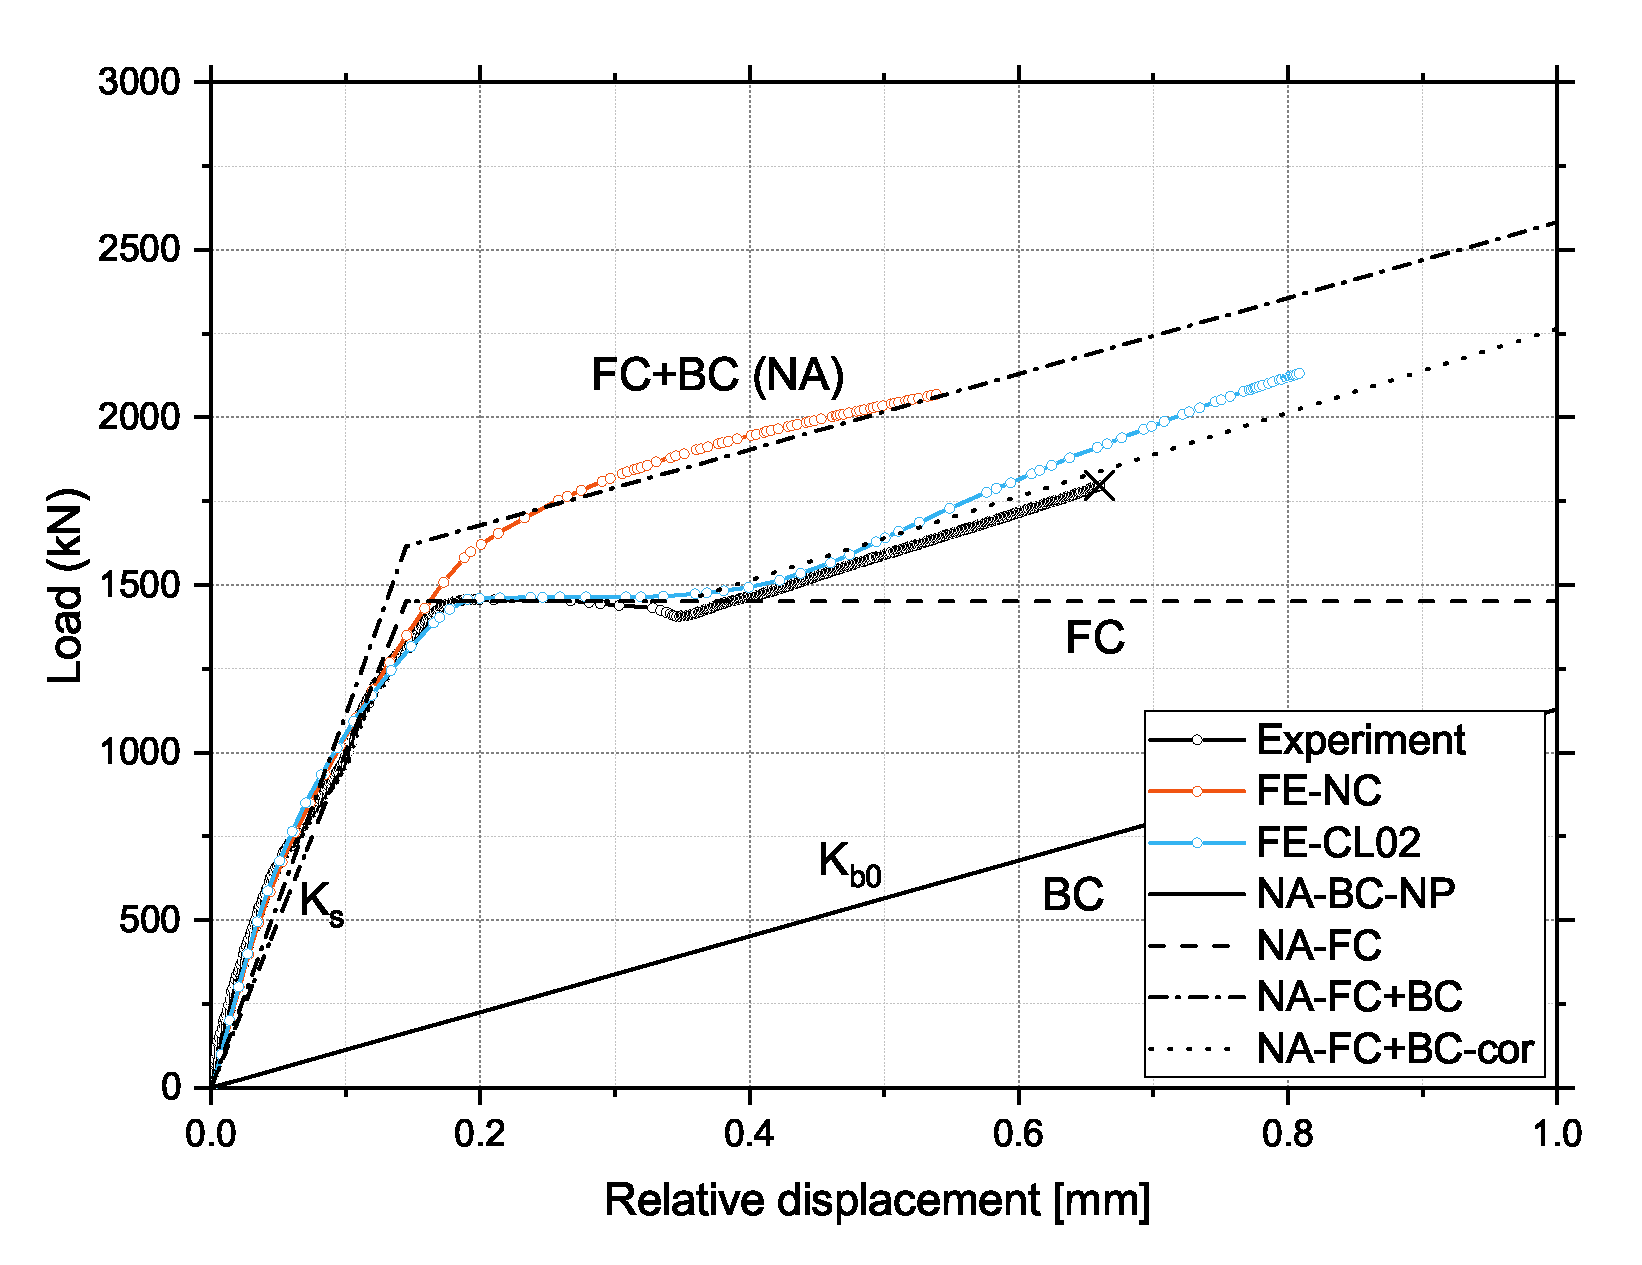
\includegraphics[width=0.7\textwidth]{imgs/ch7/rd-valid.eps}
    \caption{The relationship between load and relative displacement of experiment result, FE analysis and Numerical model}
    \label{fig-rdvali}
\end{figure}

Fig. \ref{fig-rdvali} shows the results of the finite element analysis, and the FE-NC case represents the case where the ideal state is assumed to be free of minor slips (No clearance), and it can be seen that the results of the finite element analysis are very similar to those of the theoretical numerical model, and thus it can be proved that the modeling method of the theoretical numerical model is reliable. The blue FE-CL02 represents the artificial creation of a gap of 0.2 mm between the shaft of the bolt and the hole wall (with 0.2 mm clearance), that is, the shaft of the bolt is reduced by 0.2mm compared with the original, which leads to the emergence of the tiny slip, and the joint enters into the state of bearing and transferring loads after the end of the tiny slip, which is in line with the expected behavior, and the model also indirectly proves the conjecture of the tiny gap in chapter 6, and the results of finite element analysis The finite element analysis results and the experimental results and the numerical model present almost the same mechanical behavior.